\mainmatter

\chapter{Introduzione}
 
Il basso peso alla nascita \`e una delle maggiori cause di morbilit\`a e mortalit\`a
nel periodo neonatale e nell'infanzia in tutto il mondo.
Inoltre osservazioni epidemiologiche hanno evidenziato un aumentato rischio di 
alterazioni metaboliche e malattie cardiovascolari in età adulta per i soggetti nati piccoli 
per l'et\`a gestazionale (SGA)\cite{consensus}.

Infine il 10-15\% dei bambini SGA è destinato a non raggiungere la statura normale\cite{sga}.

\section{Definizione di SGA}

In base ai dati antropometrici rilevati alla nascita, i neonati vengono classificati come:
\begin{itemize}
\item piccoli per l'epoca gestazionale (SGA - small for gestational age) quando presentano peso e/o lunghezza inferiori al 3°
   percentile o alle -2SD rispetto alle curve di normalità per sesso relative ad una popolazione di appartenenza;
\item adeguati per l'epoca gestazionale (AGA - adeguate for gestational age) quando presentano peso e/o lunghezza compresi
   fra il 3° e il 90° percentile;
\item grandi per l'epoca gestazionale (LGA - large for gestational age) quando presentano peso e/o lunghezza superiori
   al 90° percentile\cite{sga-1}.
\end{itemize}

Da ciò emerge che è necessario conoscere l'età gestazionale e disporre di standard antropometrici di riferimento per la popolazione di appartenenza, così da stabilire correttamente quando peso e/o lunghezza si collochino al di sotto del 3° percentile o siano inferiori alle -2 DS.

 Occorre notare che la definizione SGA non considera alcuni fattori di fondo che modificano la crescita, come la taglia fisica della madre,
l'etnia e la gemellarit\`a\cite{consensus}.

L'acronimo SGA è spesso erroneamente considerato sinonimo di IUGR (Intrauterine Growth Retardation), pur non essendo i due termini
equivalenti: la definizione di IUGR è primariamente di tipo ostetrico, basata su due misurazioni ecografiche che evidenzino la ridotta crescita fetale.
Un neonato che ha presentato un ritardo di crescita intrauterino non necessariamente pu\`o essere classificato come uno SGA,viceversa un
neonato SGA pu\`o essere definito IUGR. Infatti un feto che presenta un rallentamento intrauterino della crescita può collocarsi dal punto di vista 
auxologico alla nascita anche sopra le -2 DS\cite{sga}.

\section{Prevalenza dei nati SGA}

Circa il 5\% dei nati in tutto il mondo sono piccoli per l'età gestazionale, 
ma questo dato è decisamente sottostimato: nei Paesi poveri in via di sviluppo 
e del terzo mondo i neonati spesso non vengono pesati e misurati\cite{novonordisk}.

Nella regione Piemonte nell'anno 2005 sono nati 36500 bambini (fonte ISTAT); di questi 800 (2,3\%) sono SGA. Una significativa percentuale di questi bambini (10\%, ovvero 80/anno) è destinata a rimanere di statura inferiore alla norma. Per confronto altre basse stature patologiche, come da deficit di GH e sindrome di Turner, presentano un'incidenza nettamente inferiore (deficit di GH 1/3500 nati, cioè 10/anno; s. di Turner 1/2500 nate, vale a dire 15/anno). Insomma l'incidenza di bassa statura in SGA è otto volte superiore all'incidenza di bassa statura da deficit di GH e sindrome di Turner. 


\section{Cause}

Le cause del ritardo di crescita intrauterino si dividono in
fetali e materno -- placentari.


Tra le più frequenti cause fetali vi sono la gemellarità, le malformazioni congenite, le cromosomopatie e le sindromi dismorfiche: sindrome di Turner, sindrome di Cornelia de Lange, sindrome di Bloom, sindrome di Williams, trisomie dei cromosomi 13, 18, 21.
Altre cause genetiche comprendono le delezioni, le mutazioni, i polimorfismi dei geni codificanti per IGF-1,IGF-1R \cite{woods1996intrauterine} \cite{vaessen2002association} \cite{arends2002polymorphism}
e le disomie uniparentali materne dei cromosomi 14, 16, 20\cite{fowden2006imprinted}. 
Per quanto concerne queste ultime, occorre considerare che, sebbene
i geni con imprinting non rappresentino oltre lo 0,5\% dell'intero genoma, essi svolgono
però un ruolo importante nel regolare lo sviluppo fetoplacentare, controllando l'accrescimento, la 
morfologia e la capacità di scambio di nutrienti tra la placenta e il feto.
In particolare il gene IGF-2 sembra essere fortemente coinvolto nella regolazione dello sviluppo
fetoplacentare. L'importanza dell'imprinting genico è dimostrata dall'effetto della disomia uniparentale
nell'uomo e nei roditori: l'accrescimento è stimolato dalle disomie paterne, mentre \`e inibito da quelle materne.\cite{fowden2006imprinted}.
Ad esmpio il 10\% dei soggetti con sindrome di Silver Russell (condizione caratterizzata da IUGR, scarso accrescimento postnatale, asimmetria corporea e dismorfie facciali) presenta una disomia uniparentale materna del cromosoma 7. Inoltre è stato osservato che alterazioni epigenetiche del locus 11p15 (in particolare l'ipometilazione dell'Imprinting Control Region 1), che esitano nel silenziamento del gene dell'IGF-II, sono presenti nel 50\% dei soggetti con la sindrome di Silver Russell\cite{gicquel2005epimutation}.


Le cause materno -- placentari comprendono: le malattie croniche ed infettive, l'assunzione di farmaci, l'eccessivo carico di lavoro, il fumo, l'assunzione di sostanze stupefacenti, l'abuso alcolico e l'alimentazione inadeguata.

Fra le malattie croniche materne che compromettono l'accrescimento fetale vanno ricordate le cardiopatie, le patologie ematologiche, polmonari, metaboliche, renali ed autoimmuni. Per quanto riguarda le infezioni, esse rappresentano una delle più frequenti cause di iposviluppo fetale soprattutto nei paesi poveri e comprendono principalmente le infezioni appartenenti al gruppo TORCH (Toxoplasmosi, Rosolia, Citomegalovirus, Herpes Virus) e l'infezione da HIV.
Tra le cause materne vanno inclusi anche i farmaci assunti durante la gravidanza.In particolare sono da ricordare i chemioterapici, gli anticomiziali. Non vanno dimenticati gli agenti chimici, ad esempio alcuni solventi.

Bisogna considerare anche il tipo di attivit\`a lavorativa, con l'ammontare delle ore
che vi vengono dedicate durante la gestazione: \`e noto che il lavoro pesante, 
richiedente un impegno fisico importante o uno sforzo prolungato, soprattutto se nell'ultimo trimestre,
può determinare parto pretermine, eclampsia, rottura prematura delle membrane e nascita di neonati IUGR e/o SGA\cite{sga-14}.

\`E molto importante sottolineare che la gravidanza è influenzata negativamente dal fumo di sigaretta in tutta la sua evoluzione.I metaboliti del tabacco agiscono creando
una situazione di ipossia fetale soprattutto tramite due meccanismi: la formazione di carbossi -- emoglobina, 
per legame tra emoglobina e monossido di carbonio; l'aumento della secrezione di catecolamine plasmatiche
dalla midollare del surrene, che causando vasocostrizione dell'arteria uterina e di quella ombelicale riducono l'afflusso ematico al feto.
Purtroppo si tratta di un problema non irrilevante, se si considera che le donne fumatrici in gravidanza costituiscono il 23,7\% delle gestanti (sondaggio ISTAT 2001).
Il Centro Internazionale di Consultazione sul fumo ha concluso che il tabagismo durante la gestazione \`e la maggiore causa di basso peso alla nascita\cite{sga-18}.
Si \`e verificata altres\`i l'importanza del fumo passivo\cite{sga-20}. Anche l'abuso di sostanze stupefacenti e/o di alcolici agirebbe con  meccanismi analoghi a quelli sopracitati\cite{sga-24}\cite{sga-25}.

La malnutrizione materna, spesso associata ad un basso stato socio--economico, rappresenta una causa di scarso accrescimento fetale. 
Infatti \`e emerso che le donne con figli AGA presentavano una dieta più ricca in carboidrati,frutta, ferro ed acido folico rispetto a donne con figli SGA. Si è visto che è soprattutto la supplementazione di acido folico già al momento del concepimento a ridurre il rischio di avere figli piccoli per l'età gestazionale, oltre che il rischio di mielomeningocele nel nascituro.\cite{sga-26}
Inoltre alcuni lavori riportano un rischio aumentato di presentare gravidanze complicate
in donne con celiachia non diagnosticata; tale constatazione si basa sull'immunologia e 
sul background nutrizionale, poich\'e l'infiammazione del piccolo intestino causa uno
scarso assorbimento di sostanze nutritive e di conseguenza non concede al feto un apporto alimentare adeguato\cite{sga-15}.

Inoltre occorre considerare che esiste un enorme divario tra paesi in via di sviluppo e industrializzati.

Nei paesi in via di sviluppo le principali cause di dismaturità includono il fumo, l'inadeguato stato di 
nutrizione materna, la giovane età della gravida (parto prima dei 16 anni) nonché le infestazioni del Plasmodium della malaria a 
livello placentare.

Nei paesi industrializzati la nascità di bambini piccoli per l'età gestazionale
è spesso legata alla gemellarità (favorita da pratiche di fecondazione assistita
e dall'elevata età materna, superiore ai 35 anni), al fumo oppure alla dieta restrittiva e rigida della gestante.

\begin{table}[h]\centering
\begin{tabular}{cll}
\toprule
			& \multicolumn{1}{c}{Paesi sviluppati}			& \multicolumn{1}{c}{Paesi in via di sviluppo} \\
\midrule
Fetali & Gemellarit\`a  			& Infezioni			\\
 & (da fecondazione assistita) & \\\midrule
\multirow{4}{*}{Materno -- placentari} & Fumo						& Fumo/povertà		\\\cmidrule(l){2-3}
			& Dieta restrittiva e rigida	& Inadeguata nutrizione\\
			& &  materna \\\cmidrule(l){2-3}
			& Avanzata età materna  &	Giovane età materna \\\cmidrule(l){2-3}
			& Disfunzioni placentari	& Eccessivo carico di lavoro	\\\bottomrule
\end{tabular}
\label{tab-cause}
\caption{Cause di iposviluppo fetale in correlazione al paese di origine.}
\end{table}

Come vediamo i bambini SGA costituiscono un gruppo eterogeneo per eziologia.

Dal punto di vista clinico è importante una suddivisione che consideri la diversa compromissione delle principali variabili antropometriche: peso,lunghezza e circonferenza cranica.

La maggior parte degli individui SGA (80\%) presenta alla nascita il peso ridotto, ma la lunghezza e la circonferenza cranica sono normali o solo lievemente ridotti.
In questo caso la noxa (gestosi, malattie, malnutrizione materna) agisce piuttosto tardivamente, dopo la ventiseiesima settimana di gestazione e compromette soprattutto la biometria addominale: in condizioni di scarso afflusso sanguigno viene privilegiato lo sviluppo degli organi nobili (cervello, cuore, surrene) a scapito della massa epatica, che va incontro ad ipotrofia cellulare. 
Qusta situazone porta ad un ritardo di crescita disarmonico (SGA asimmetrico), con prevalente deficit ponderale.

Le cause fetali (in particolare le alterazioni genetiche e le sindromi cromosomiche) o l'insufficienza utero-placentare severa ad esordio 
precoce, vale a dire prima della sedicesima settimana di gestazione,oltre a gravi infezioni materne, farmaci e fumo  hanno un impatto pi\'u importante sullo sviluppo fetale, comportando un'ipocellularità con riduzione sia della circonferenza addominale, che della lunghezza degli arti e della circonferenza cranica. In tal caso si parla di SGA simmetrico, altrimenti detto "`low profile"' o armonico, caratterizzato da ridotta lunghezza, deficit ponderale e circonferenza cranica inferiore alla norma (20\% dei bambini SGA).

La distinzione fra SGA asimmetrici e simmetrici \`e importante: studi osservazionali 
hanno dimostrato che i bambini con deficit prevalentemente ponderale alla nascita 
(SGA asimmetrici) presentano una migliore prognosi staturale rispetto agli SGA simmetrici.\cite{sga-10}

\section{Complicanze}

Nel tempo i nati SGA presentano oltre alla bassa statura anche alterazioni endocrino--metaboliche e cardiovascolari. 
Per spiegare tali complicanze è stato proposto il modello del fenotipo risparmiatore (\textit{Thrifty phenotype}).
Secondo questa ipotesi, la malnutrizione intrauterina sarebbe il fattore scatenante
per innescare nel feto una serie di meccanismi di adattamento indispensabili per 
la sua sopravvivenza a breve termine, ma che comportano delle modificazioni permanenti
del metabolismo energetico.
Tali meccanismi di adattamento avvengono per favorire lo sviluppo dei tessuti 
nobili come quello nervoso, cardiaco e renale, a scapito dei tessuti adiposo ed endoteliale .

In particolare sembrerebbe instaurarsi una riduzione della sensibilità all'insulina
a livello periferico condizionante il calo della glicogenesi e della lipogenesi
con raggiungimento di livelli plasmatici ottimali di glucosio e acidi grassi liberi
indispensabili per un corretto sviluppo del sistema nervoso e degli organi splacnici.\cite{sga-51}



\`E possibile distinguere conseguenze a breve e lungo termine che tale risposta
adattativa produce nei soggetti coinvolti.

Tra le ripercussioni immediate la più importante riguarda lo scarso accrescimento
staturo-ponderale presente sia a livello intrauterino che post nascita. Inoltre 
il nato piccolo per l'età gestazionale tende ad accumulare grasso in depositi a livello
viscerale a discapito di una corretta formazione di massa magra. L'accelerazione e 
l'attivazione anticipate di processi fisiologici costituiscono un ulteriore tipo di 
effetto a breve termine: spesso si assiste alla ricerca di un tempo gestazionale
rapido (prematurità) al fine di ridurre la permanenza in un ambiente stressante
e non ottimale per l'accrescimento\cite{sga-53}; successivamente soprattutto nelle bambine si possono manifestare pubarca precoce e pubertà anticipata e/o a rapida progressione. 

Le conseguenze a lungo termine comprendono malattie della sfera glicometabolica (ridotta sensibilità insulinica, diabete mellito,
ipertensione arteriosa, sovrappeso e obesità) secondarie all'alterato sviluppo dei tessuti pancreatico, endoteliale ed adiposo.\cite{sga-32}


\section{Crescita nei bambini SGA: storia naturale}

Le misure alla nascita sono determinate principalmente dalle condizioni ambientali in utero. Successivamente, nei primi 12-18 mesi di vita extra-uterina, le differenze in peso e lunghezza determinate dalle condizioni prenatali sono ridotte, mentre aumenta la variabilità legata al patrimonio genetico. Pertanto in questo periodo gli individui nati piccoli da genitori di alta statura tendono a crescere di più, mentre quelli nati grandi da genitori di bassa statura tendono a crescere meno. 


La velocità di crescita è molto alta subito dopo la nascita: nei maschi la lunghezza aumenta nei primi 3 mesi ad una velocità di circa 40 cm/anno; successivamente questa velocità diminuisce gradualmente raggiungendo i 14 cm/anno fra l'età di 9 mesi e 1 anno. La velocità di crescita ponderale presenta il proprio picco fra il primo e il secondo mese di vita dopo la nascita, poi segue una graduale riduzione; così la velocità iniziale di circa 10 kg/anno scende a 3 kg/anno tra l'età di 9 e 12 mesi. Tra l'età di 2 e 4-5 anni la velocità di crescita staturale diminuisce progressivamente\cite{tanner1994growth}.
 All'età di 5 anni il bambino entra in una fase di latenza. In questo periodo la statura aumenta di circa 5 cm/anno. In pubertà il corpo incomincia a crescere ad alta velocità e la statura può aumentare di 10 cm nell'anno centrale di scatto puberale per i maschi e di 8 cm per le femmine. Si tratta di velocità comunque inferiori rispetto a quelle riscontrabili nei primi due anni di vita.
 La figura 1.1 illustra l'andamento di crescita nei diversi periodi di vita evolutiva.
 
\begin{figure}[!h]
  \begin{center}
      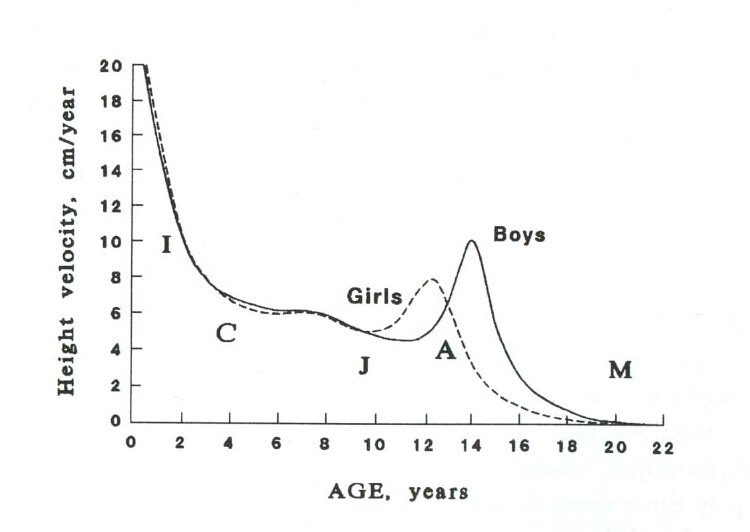
\includegraphics{grafici/grafico_velocita} %\\
  \end{center}
  \caption{Curve di velocità di crescita staturale per maschi e fammine sani.\\I: prima infanzia, C: seconda infanzia, J: terza infanzia, A: pubertà, M: età adulta. \cite{bogin1996evolution}}
  \label{fig:GraficoVelocita}
\end{figure}
 
 Pertanto la crescita di recupero (\textit{catch up growth}) ha più successo quando avviene nei primi due anni di vita. La crescita di recupero è un accrescimento superiore al normale che segue un periodo di restrizione e che compenserà almeno in parte il deficit di crescita causato da condizioni patologiche \cite{boersma1997catch}.
La crescita di recupero è attesa ad esempio dopo la correzione di deficit di GH, malnutrizione, malattia celiaca o ipotiroidismo. Inoltre ci si aspetta che avvenga anche nella maggior parte dei bambini nati piccoli per l'età gestazionale (SGA). I meccanismi che si celano dietro questa crescita compensatoria non sono chiari, ma studi sperimentali sulla restrizione di crescita suggeriscono che un temporaneo arresto della senescenza dei condrociti della cartilagine di accrescimento potrebbe essere uno dei meccanismi 
coinvolti.
La teoria si basa sull'ipotesi che la cartilagine di accrescimento abbia una sua storia replicativa, assumendo un limite alla capacità proliferativa dei condrociti. Una temporanea condizione avversa, rallentando il tasso di crescita dei condrociti, ne postporrebbe la senescenza.\cite{gafni2001catch} 


Il 90\% dei neonati SGA presenta crescita di recupero entro i primi due anni di
vita\cite{karlberg1995growth}. Ciò permette loro di raggiungere una statura normale, non media. Infatti la statura media degli adulti nati SGA è di circa 1 DS al di sotto della statura 
media della popolazione generale\cite{leger1997reduced}. Secondo i centili italiani di riferimento \cite{cacciari2006italian} la statura media della popolazione generale corrisponde a 163 cm per le femmine ed a 176 cm per i maschi. Considerando che la statura media dei nati SGA è 1 DS inferiore rispetto alla statura media della popolazione generale,   
si ottiene che la statura media per un individuo italiano nato SGA è di 157 cm per le femmine e di 170 cm per i maschi. 


Il 10\% degli individui nati SGA non raggiunge la statura normale, cioè presenta un'altezza finale inferiore alle -2 DS, vale a dire al di sotto dei 151 cm per le femmine ed inferiore ai 164 cm per i maschi. 
Le cause di bassa statura nei soggetti SGA comprendono: mancata o incompleta crescita di recupero; pubertà sovente anticipata e a rapida progressione; scatto puberale di crescita ridotto; maturazione scheletrica inizialmente ritardata seguita da rapida accelerazione.
 

La crescita di recupero è assente o incompleta negli individui nati SGA per lunghezza. In particolare è stato stimato che il rischio relativo di bassa statura all'età di 18 anni tra i bambini nati SGA è 5,2 per quelli 
piccoli in peso e 7,1 per quelli piccoli in lunghezza. \cite{cianfarani2006hormonal}. Anche l'eventuale presenza di un quadro sindromico (ad esempio la sindrome di Silver Russell) riduce le probabilità di recupero staturale. Un'altra importante variabile che condiziona la crescita di recupero è la statura dei genitori: i bambini SGA nati da genitori bassi generalmente non presentano un soddisfacente recupero staturale. Anche la grave prematurità, così come le anomalie genetiche/i polimorfismi dell'asse GH--IGF-1 influenzano negativamente la crescita di recupero. 


Un'altra causa di bassa statura nei soggetti nati SGA è la pubertà sovente anticipata e/o a rapida progressione\cite{albertsson2000children}.
Come evidenziato dagli studi osservazionali di Prader\cite{gasser1985human}
, Stanhope%citare 
e Largo%citare 
 l'altezza finale dipende prevalentemente dalla velocità di crescita prepuberale nei maschi, nelle femmine anche dalla durata di crescita prepuberale: è stato stimato che le ragazze hanno realizzato circa l'85\% ed i ragazzi circa il 90\% della statura definitiva all'ingresso in pubertà. Il guadagno in statura che si ottiene durante lo scatto puberale è legato più alla durata dello scatto,che alla sua intensità. Ciò significa che se l'individuo anticipa la pubertà sottrae tempo alla crescita prepuberale e dunque centimetri significativi per la sua statura finale. Se inoltre la pubertà del soggetto è rapida progressione viene meno l'ultima possibilità per migliorare l'altezza definitiva, poichè viene ridotta la durata dello scatto puberale.
 

Per quanto concerne la maturazione scheletrica, i bambini SGA tendono ad avere un'età ossea modicamente ritardata (anche di due anni) fino all'epoca puberale. Dunque una previsione della statura definitiva basata sull'età ossea e fatta in età prepuberale potrebbe fornire risultati rassicuranti. Tuttavia l'inizio anticipato della pubertà e la successiva accelerazione dello sviluppo puberale associato a rapida maturazione scheletrica determinano un crollo della previsione e, sopratutto, della effettiva statura finale\cite{job1986histoire}.

Il raggiungimento di una statura inferiore alla norma (vale a dire al di sotto di -2DS)è un evento più comune nella popolazione nata SGA che negli individui con peso alla nascita adeguato, come dimostrato da uno studio a lungo termine condotto su 213 soggetti SGA e 272 con peso alla nascita normale. Questo studio ha evidenziato che il 
13,6\% degli individui nati SGA presentava una statura inferiore a -2 DS all'età di
20-21 anni, contro solo l'1.8\% del gruppo di controllo.\cite{leger1997reduced}

I soggetti nati SGA costituiscono una componente importante degli adulti di bassa statura (25\%)e rappresentano una popolazione destinata ad aumentare numericamente se si considerano i fattori di rischio per la nascita di bambini SGA .

Va notato che una bassa statura persistente può associarsi ad una significativa alterazione degli aspetti psico-sociali. In particolare un recente studio condotto sulla popolazione generale del Regno Unito ha dimostrato l'impatto negativo che una bassa statura può esercitare sulla qualità della vita, intesa come benessere fisico, psicologico e sociale\cite{christensen2007evaluation}. 
